%&pdflatex

\documentclass[12pt]{article}

\usepackage[spanish, es-tabla]{babel}
\usepackage{enumerate}
\usepackage{lscape}
\usepackage{vmargin}
\usepackage{pdfpages}
\usepackage{fancyhdr}
\usepackage{graphicx}
\usepackage{float}
\usepackage{titlesec}
\usepackage[bottom]{footmisc}
\usepackage[hidelinks]{hyperref}
\usepackage{listings}
\usepackage{color}
\usepackage{colortbl}
\usepackage{xcolor}
\usepackage{amsmath}
\usepackage{array}
\usepackage{svg}
\usepackage{pgfgantt}
\usepackage[T1]{fontenc}
\usepackage[sfdefault]{AlegreyaSans} %% Option 'black' gives heavier bold face
%% The 'sfdefault' option to make the base font sans serif
\renewcommand*\oldstylenums[1]{{\AlegreyaSansOsF #1}}


%*******************************************************************************
\extrarowheight = -0.3ex
\renewcommand{\arraystretch}{2.25}
\setpapersize{A4}
\hypersetup{
    colorlinks=true,
    linkcolor=blue,
    urlcolor=purple,
    citecolor=black, 
    linktocpage=true,
}
\definecolor{gray95}{gray}{.95}
\definecolor{gray75}{gray}{.75}
\definecolor{barblue}{RGB}{153,204,254}
\definecolor{groupblue}{RGB}{51,102,254}
\definecolor{linkred}{RGB}{165,0,33}
\lstset{
    frame=Ltb,
    framerule=0pt,
     aboveskip=0.5cm,
     framextopmargin=3pt,
     framexbottommargin=3pt,
     framexleftmargin=0.4cm,
     framesep=0pt,
     rulesep=.4pt,
     backgroundcolor=\color{gray95},
     rulesepcolor=\color{cyan},
     %
     stringstyle=\ttfamily,
     showstringspaces = false,
     basicstyle=\small\ttfamily,
     commentstyle=\color{cyan},
     keywordstyle=\bfseries\color{purple},
     %
     numbers=left,
     numbersep=15pt,
     numberstyle=\small,
     numberfirstline = false,
     breaklines=true,
}

%minimizar fragmentado de listados
\lstnewenvironment{listing}[1][]
   {\lstset{#1}\pagebreak[0]}{\pagebreak[0]}


\lstdefinestyle{C}
   {
       language=C++,
   }

\lstdefinestyle{python}
    {
        language=Python,
    }

\setcounter{secnumdepth}{4}
%*******************************************************************************
%   Adding a new level of section --> subsubsubsection
%******************************************************************************
\titleclass{\subsubsubsection}{straight}[\subsection]

\newcounter{subsubsubsection}[subsubsection]
\renewcommand\thesubsubsubsection{\thesubsubsection.\arabic{subsubsubsection}}
\renewcommand\theparagraph{\thesubsubsubsection.\arabic{paragraph}} % optional; useful if paragraphs are to be numbered

\titleformat{\subsubsubsection}
  {\normalfont\normalsize\bfseries}{\thesubsubsubsection}{1em}{}
\titlespacing*{\subsubsubsection}
{0pt}{3.25ex plus 1ex minus .2ex}{1.5ex plus .2ex}

\makeatletter
\renewcommand\paragraph{\@startsection{paragraph}{5}{\z@}%
  {3.25ex \@plus1ex \@minus.2ex}%
  {-1em}%
  {\normalfont\normalsize\bfseries}}
\renewcommand\subparagraph{\@startsection{subparagraph}{6}{\parindent}%
  {3.25ex \@plus1ex \@minus .2ex}%
  {-1em}%
  {\normalfont\normalsize\bfseries}}
\def\toclevel@subsubsubsection{4}
\def\toclevel@paragraph{5}
\def\toclevel@paragraph{6}
\def\l@subsubsubsection{\@dottedtocline{4}{7em}{4em}}
\def\l@paragraph{\@dottedtocline{5}{10em}{5em}}
\def\l@subparagraph{\@dottedtocline{6}{14em}{6em}}
\makeatother

\setcounter{secnumdepth}{4}
\setcounter{tocdepth}{4}

%*****************************************************************************

\begin{document}

  \begin{titlepage}
    \centering
   {\bfseries\Large Universidad Carlos III de Madrid \par}
    \vspace{5cm}
    {\scshape\Huge Informe del Trabajo de Evaluación del Bloque 2 \par}
    \vspace{2cm}
    {\itshape\Large Diseño de circuitos electrónicos para comunicaciones}
    \vfill
    {\Large Autores: \par}
    \vspace{1cm}
    {\Large Markel Serrano y Daniel Theran}
    \vfill
    {\Large 20 de Noviembre del 2022 \par}
  \end{titlepage}

  %\tableofcontents
  %\newpage
  
  \section{Apartado 1}
    \paragraph*{}
    En el primer apartado se pide calcular la SNR a la entrada y la salida del LNA del circuito para dos valores de entrada dados, -30 y -70 dBm.
    Para ello, y como puede verse en los cálculos anexados, primero debe calcularse la SNR de entrada del LNA. Para ello, se divide la potencia
    de la señal de entrada entre la potencia del ruido térmico a la entrada, como puede verse en la fórmula, y se cambia de unidades lineales a logarítmicas.
    
    \paragraph*{}
    Una vez calculada la SNR de entrada para ambos casos, basta con restar la figura de ruido del LNA para obtener las señales SNA de salida correspondientes.


  \section{Apartado 2}
  \paragraph*{}
  En el segundo apartado se pide calcular la figura de ruido del mezclador y etapas siguientes para que la figura de ruido total del receptor no supere nunca 10dB.
  Como puede verse en el diagrama de bloques anexado, se ha modelado el circuito con una bifurcación en dos líneas (la línea I y la Q, como corresponde a un receptor en cuadratura).
  Ambas líneas son simétricas exceptuando un desfase de 90º, pero los bloques que las componen son los mismos. Más concretamente, cada línea se compone
  de un mezclador, un filtro paso bajo y un controlador automático de ganancia (AGC).
  \paragraph*{}
  Para resolver este apartado, se ha de tener en cuenta que la figura de ruido más importante, debido a la formula de Friis, es la del LNA, la cual es conocida (de 2,4 dB).
  Por tanto, pueden modelarse el resto de bloques como uno solo, y encontrar la figura de ruido máxima de este simplemente despejando de la formula de Friis. Así,
  se consigue una figura de ruido máxima posible para ese bloque equivalente de 25,18 dB.

  \section{Apartado 3}
  \paragraph*{}
  En el tercer apartado se pide calcular las ganancias mínima y máxima del AGC, suponiendo el caso de máxima ganancia para -70 dBm a la entrada.
  Sabiendo que el AGC mantiene una salida 1 Vrms, y que su margen de ganancias es de 40 dB, basta con calcular la ganancia máxima, que será de 130 dBm
  (la diferencia entre los 60 dbM a la salida correspondientes a 1 Vrms y la suposición de -70 dBm de la entrada.) Después, se aplica el rango de 40 dB que
  caracteriza al AGC y se obtiene la ganancia mínima, de 90 dB para este caso.
  \section{Apartado 4}
  \paragraph*{}
  El cuarto apartado se pide diseñar un AGC lineal en dB con un detector de valor rms, y calcular la tensión de referencia necesaria.
  Para ello, se diseña primero un diagrama de bloques lineal en el que se introduce un detector de envolvente, un bloque de paso a potencia,
  un mezclador para introducir la tensión de referencia y un integrador. Así, pasando este diagrama de bloques lineal a logarítmico, despejamos primero
  la ecuación que relaciona la entrada Vi con la salida Vo para despejar la Ley de Control y después se despeja la ecuación del mezclador que relaciona nuestro
  tono de prueba con Vo. De esta forma, y analizando dicho caso en régimen permanente, encontramos que la tensión de prueba necesaria para mantener la salida dada es de 3 dB (es decir, 
  1,41 Vrms).
  \section{Apartado 5}
    
  \section{Apartado 6}

  \section{Anexo: Desarrollo de los cálculos utilizados}

  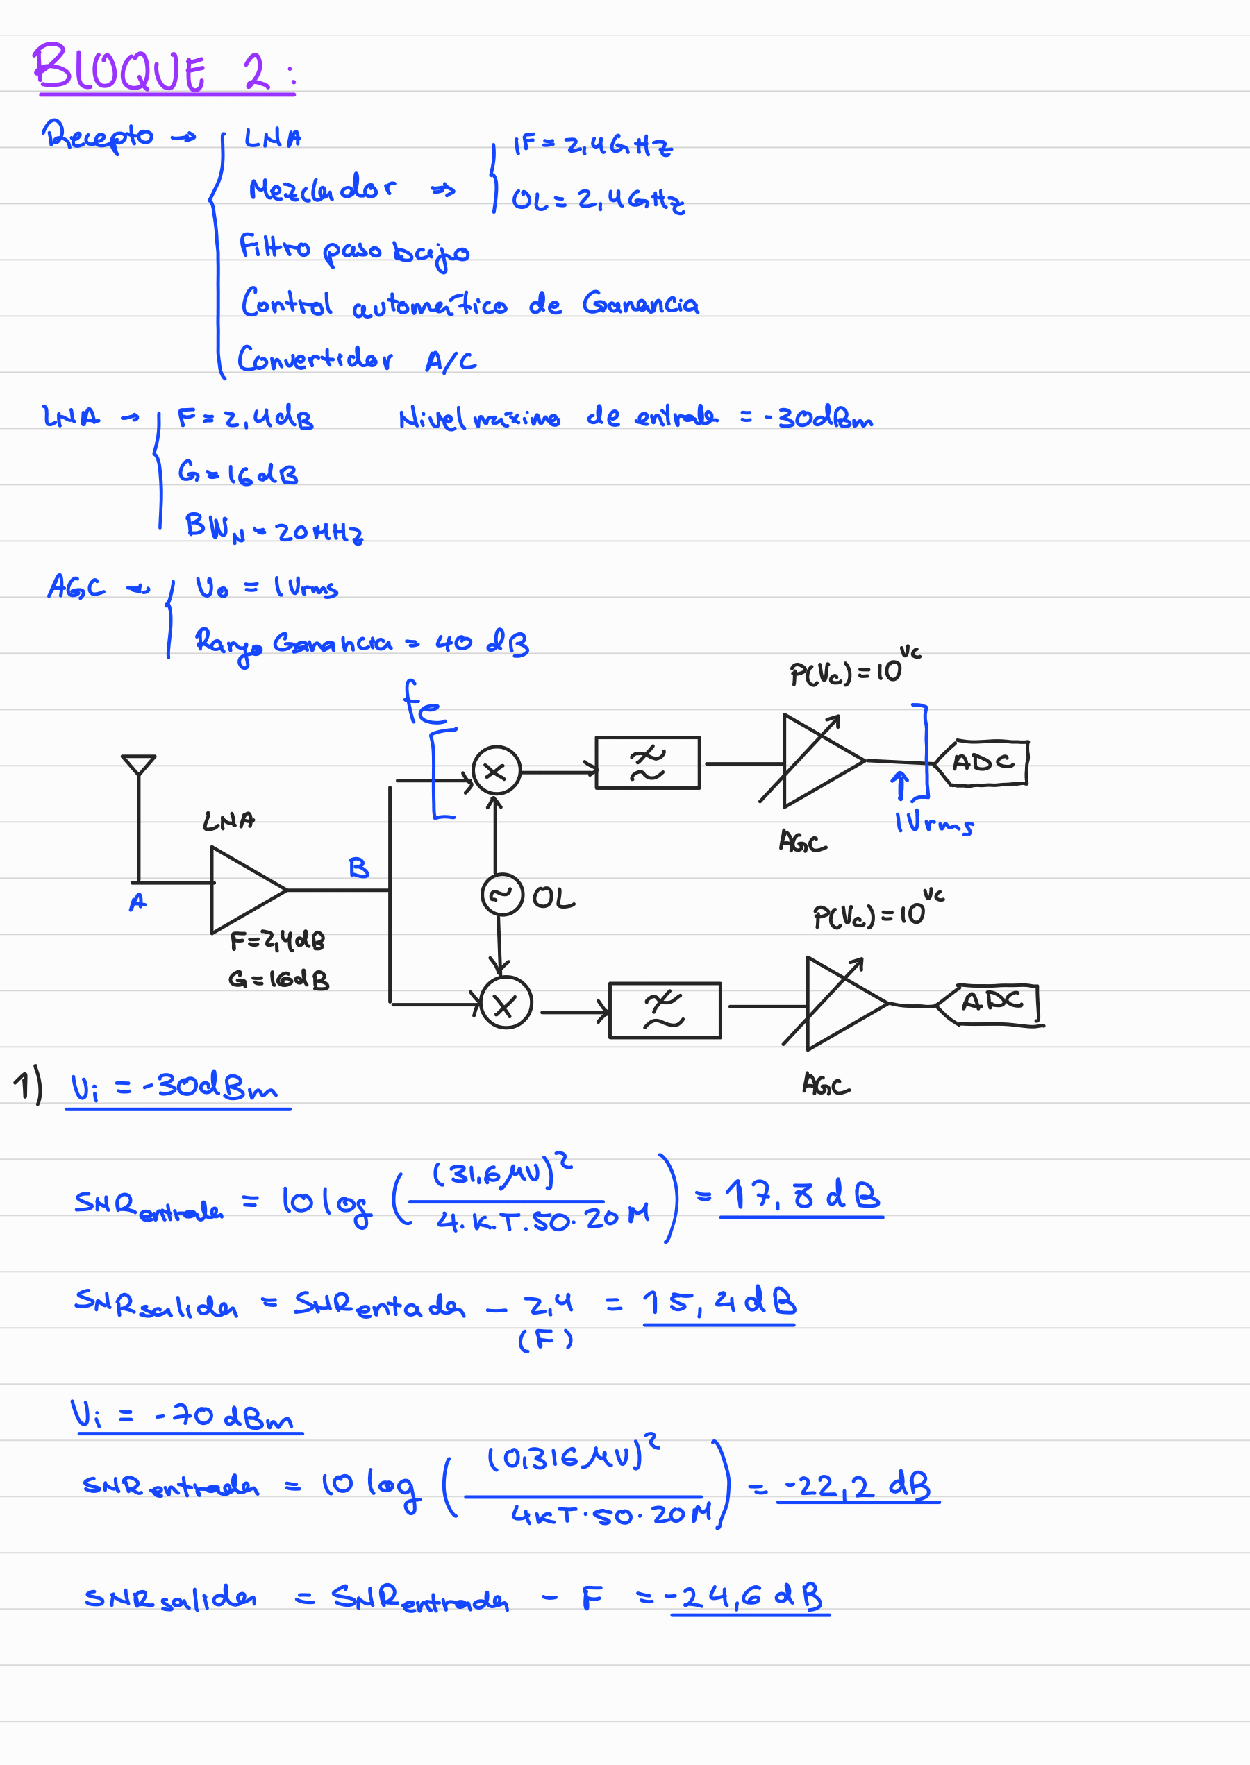
\includepdf[pages=-,pagecommand={},width=1.4\textwidth,offset= 2.5cm -2cm]{img/Ejercicio_Bloque_2.pdf}
  
 
\end{document}
